\input{../../input/main}

\begin{document}

\begin{center}
  \Large{\textbf{Городской центр физического образования, 10 класс.}\\
  \textit{Серия 16Ш, 19 февраля 2015.}}
\end{center}

\begin{center}
  \Large\textbf{ Напряжённость и потенциал. }
\end{center}

\large

\task{ Медный шарик диаметра $d=1$ см движется с постоянным ускорением
  $a=100 \mbox{ см/с}^2$. Найдите напряжённость поля в центре
  шарика. Какова максимальная разность потенциалов между точками этого
  шарика? Масса электрона $9 \cdot 10^{-31}$ кг, заряд электрона
  $1{,}6 \cdot 10^{-19}$ Кл. }
% Зильберман, ШФО, 5.4

\task{ Электрон и позитрон движутся по окружности вокруг своего
  неподвижного центра масс, образуя атом позитрония. Найти отношение
  потенциальной и кинетической энергий частиц. Электрон и позитрон
  отличаются только знаками заряда. }
% НГУ-1, 3.15

\taskpic{ Скорости двух электронов $v_1$ и $v_2$ лежат в одной
  плоскости и при расстоянии $l$ между электронами образуют углы
  $\alpha$ с прямой, соединяющей электроны. На какое минимальное
  расстояние сблизятся электроны, если скорости $v_1$ и $v_2$ равны по
  модулю $v$? Заряд электрона равен $e$, масса равна $m$. }
{
  \begin{tikzpicture}
    \draw[thick,*-*] (0,0) node[below] {$e$} -- (3.5,0) node[below]
    {$e$}; 
    \draw[thick,->] (0,0) -- ++(40:1.5cm) node[above,blue]
    {$\vec{v}_1$};
    \draw[thick,->] (3.5,0) -- ++(140:1.5cm) node[above,blue]
    {$\vec{v}_2$};
    \draw (0,0) ++(20:0.75cm) node[blue] {$\alpha$};
    \draw (3.5,0) ++(160:0.75cm) node[blue] {$\alpha$}; 
  \end{tikzpicture}
}
% НГУ, 3.18

\task{ Два шарика с зарядами $+q$ и $-q$ одинаковой массы $m$,
  соединнёных невесомым стержнем длины $l$, движутся по окружности в
  однородном электрическом поле напряжённости $\vec{E}$. В тот момент,
  когда стержень направлен вдоль вектора $\vec{E}$, заряды имеют
  скорость $v_0$. Найти силу натяжения стержня в момент, когда он
  повернулся на $\pi/2$. Силой тяжести пренебречь.  }
% НГУ-1, 3.21
\begin{center}
  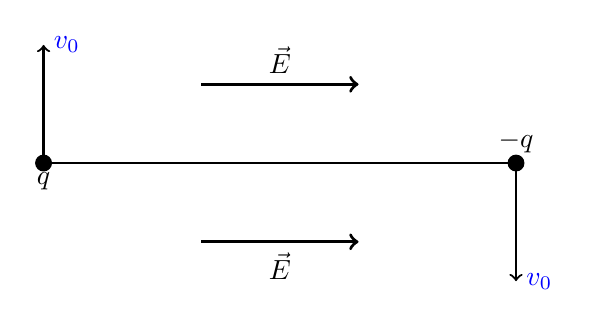
\begin{tikzpicture}
    \draw[thick] (0,0) -- (6,0);
    \draw[thick,->] (0,0) -- ++(up:1.5cm) node[right,blue] {$v_0$};
    \draw[thick,->] (6,0) -- ++(down:1.5cm) node[right,blue] {$v_0$};
    \draw[fill=black] (0,0) circle (0.1cm) node[below] {$q$};
    \draw[fill=black] (6,0) circle (0.1cm) node[above] {$-q$};
    \draw[very thick,->] (2,1) -- (4,1) node[midway, above] {$\vec{E}$};
    \draw[very thick,->] (2,-1) -- (4,-1) node[midway, below] {$\vec{E}$}; 
  \end{tikzpicture}
\end{center}

\end{document}


%%% Local Variables: 
%%% mode: latex
%%% TeX-engine:xetex
%%% TeX-PDF-mode: t
%%% End:
